\documentclass[11pt,oneside,a4paper]{book}
\usepackage[utf8]{inputenc}
\usepackage{amsmath}
\usepackage{graphicx}
\usepackage[spanish]{babel}
\usepackage{titlesec}
\usepackage[section]{placeins}
\usepackage{float}
\usepackage{url}
 
\titleformat{\chapter}[display]
  {\normalfont\bfseries}{}{0pt}{\Huge}
  
\usepackage{lipsum} 
\title{Agentes físicos y Robocup}
\author{Marcos Esteve Casademunt y Jose Gómez Gadea}

\date{Junio 2018}
\makeindex
\begin{document}

\maketitle
\tableofcontents
\listoffigures
\chapter{Resumen}
El RoboCup parte de la idea de conseguir que unos robots (agentes) sean capaces de jugar al fútbol y lleguen a alcanzar a los humanos en este deporte (como ya sucedió con el ajedrez en 1997). Esta competición, practicada por grupos de todas las edades, consiste en crear la mejor inteligencia artificial y portarla a un entorno real y físico donde los agentes puedan competir entre ellos. Esta competición ha llegado a extenderse a diversas categorías que engloban distintos tamaños de robots, e incluso se han llevado a competiciones en entornos simulados.

Actualmente, en los agentes físicos existen problemas al intentar portar al mundo real su software pese a haber sido ya testeado en un entorno simulado. Esto es debido a la gran cantidad de variables que se dan en el mundo real y la complejidad de ser simuladas en un entorno virtual. A lo largo de este trabajo hablaremos de los componentes básicos y teóricos de estos agentes y de los principales problemas que pueden surgir al portarlos al mundo real. Todo esto lo veremos con el RoboCup como principal ejemplo. Además intentaremos aportar otros ejemplos prácticos que se están desarrollando actualmente. 

\chapter{Introducción}
\section{¿Qué es un agente físico?}
Para comenzar, será necesario definir el significado de agente físico. Un agente físico es un agente situado en un entorno real y físico. Estos agentes estarán compuestos por un conjunto de sensores, actuadores y una capacidad cognitiva que les permitirá evaluar, decidir y colaborar para conseguir el objetivo propuesto. Por ejemplo, en nuestro caso de estudio; los robots del RoboCup Rescue tienen un conjunto de sensores que les permiten observar el mundo, un conjunto de actuadores que le permiten interactuar con él, y una “mente” que les permite interrelacionar los sensores con los actuadores generando un plan y de esta forma conseguir el rescate de la persona, la retirada de escombros, etc. En los puntos posteriores ahondaremos más en el RoboCup.
\section{Problemática de un agente físico}
En los agentes definidos anteriormente tenemos un conjunto de problemas que siguen siendo un gran quebradero de cabeza. Se dan mayoritariamente en el software, por lo cual los programadores deben de tenerlos muy en cuenta sobretodo a la hora de definir la base del agente. Los problemas más relevantes son:

\textbf{Acceso continuo a datos.}	En el entorno de un agente físico se producen cambios continuamente. Esto provoca la necesidad de estar constantemente analizando los datos que entran por los distintos sensores. Estos cambios se pueden producir a una velocidad mucho mayor de la que es capaz de procesar el agente, por lo que será necesario saber qué datos son importantes y cuáles deben ser descartados.

\textbf{Gestión del tiempo global}. Para que este sistema distribuido trabaje correctamente, será necesario que todos los sensores y componentes trabajen al unísono. Para ello debemos definir una unidad de tiempo que indicará a todos los sensores cuándo tienen que actuar y así todos los componentes trabajar sobre el mismo instante de tiempo. Se suele utilizar un reloj global que marca dicha frecuencia.

\textbf{Comunicación en tiempo real}. Al tratarse de un sistema distribuido, al tiempo de procesamiento se le suman los tiempos de comunicación entre los sensores, la unidad de control y los actuadores. Este tiempo deberá ser lo suficientemente reducido para poder reaccionar correctamente a los eventos producidos en el entorno.

\textbf{Gestión de los recursos}. Otro de los problemas en los agentes físicos es que la capacidad de su hardware es reducida. Esto hace que se necesite un estricto control de los procesos que se están ejecutando en cada momento sobre los componentes, dando prioridad a aquellos procesos más importantes sin dejar de lado a los demás procesos. Para esto necesitaremos un algoritmo o sistema capaz de gestionar las prioridades.

\textbf{Tolerancia a fallos}. Es posible que se dé una situación en el agente que no haya sido contemplada. Cuando se da una situación como esta, es necesario que el sistema sea capaz de recuperarse del posible fallo provocado por esta situación sin la necesidad de abortar ningún proceso.



\section{Agentes en tiempo real}
Como hemos comentado anteriormente, uno de los factores más comprometidos en el desarrollo de agentes físicos es el tiempo, ya que se da la necesidad de que dichos agentes sean en tiempo real para que su ejecución en el mundo físico sea posible.


Que los agentes sean en tiempo real consiste en que las acciones que estos tomen van a depender mayoritariamente del entorno al que están siendo sometidos en ese mismo momento y actuar acorde a ello. En caso de que dicho entorno cambie, las nuevas acciones del agente se agregaran a las anteriores. También es habitual que se lleguen a detener las acciones que ya se estaban llevando a cabo para sustituirlas por otras más actualizadas.

Dado las altas restricciones temporales que existen en estos agentes, será necesaria una arquitectura que permita operar con ellos de manera adecuada. Como ejemplo, podemos utilizar ARTIS, la cual consiste en una arquitectura vertical por capas utilizada para sistemas que tengan que operar en entornos en tiempo real. Esta arquitectura está formada por:


\begin{list}{•}{}
\item Un conjunto de sensores y actuadores  que permiten al agente interactuar con el entorno.	
\item Un conjunto de creencias que definen el conocimiento del mundo.
\item Un conjunto de comportamientos que definen la forma en la que el agente interactúa con el entorno 
\item Un módulo de control, que es el responsable de la ejecución en tiempo real del sistema. 
\end{list}


\chapter{Robocup}
\section{Objetivos}
El RoboCup es un intento de promocionar la investigación en IA y robótica mediante una competición en la cual los participantes compiten con sus robots para ganar una partida de soccer (fútbol), planificar y realizar operaciones de rescate como ocurre en la RoboCup Rescue, o otras nuevas modalidades que han aparecido más recientemente. Esta competición permite probar y evaluar distintos algoritmos, teorías y arquitecturas como la que ya hemos comentado en el apartado anterior.
\section{Datos Técnicos}
Una de las razones por las cuales el RoboCup resulta interesante para investigadores de todo el mundo es la necesidad de integrar una amplia gama de tecnologías en un mismo agente, lo cual es algo necesario en esta competición para obtener las mejores respuestas a las situaciones dadas.

En la RoboCup tenemos dos formas principales de competir; una en un entorno virtual, y otra en un entorno físico.
\begin{figure}[H]
\begin{center}
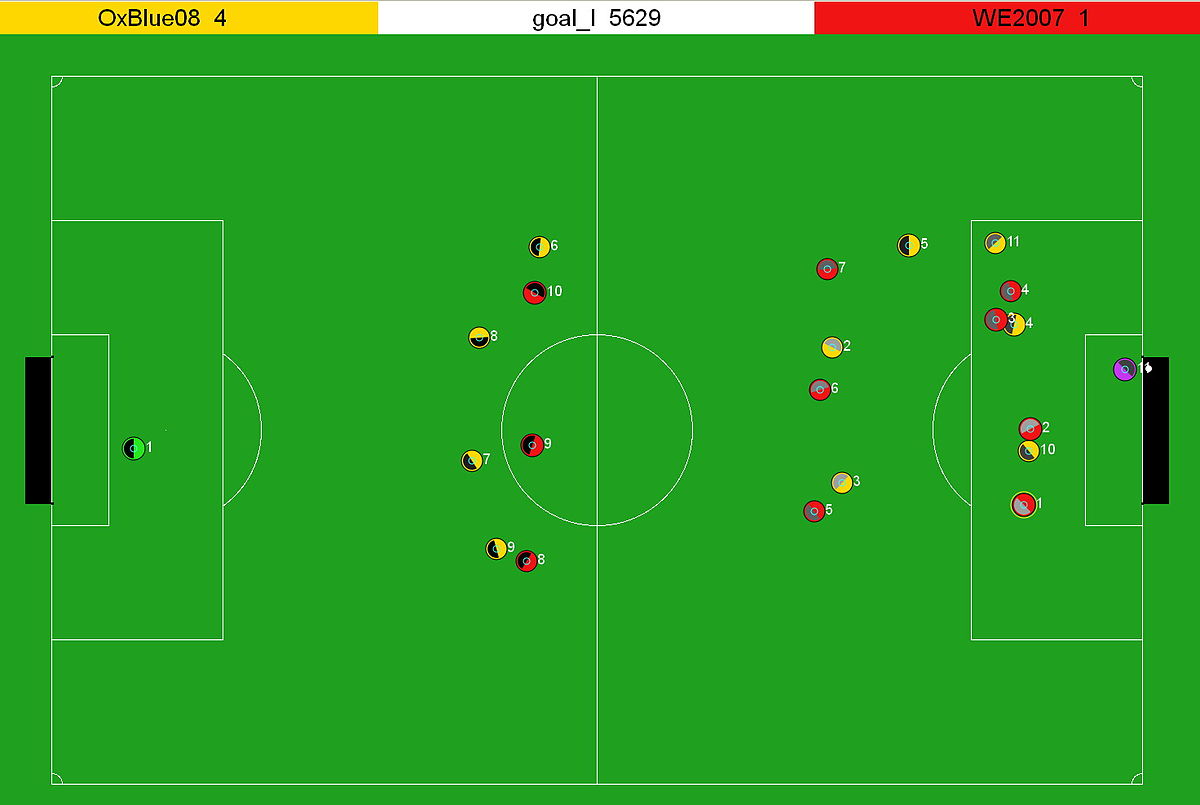
\includegraphics[scale=0.25]{Images/2.jpg}
\caption{Entorno virtual del RoboCup}
\end{center}
\end{figure}
En el caso del entorno virtual [2], los agentes disponen de un entorno controlado que les aporta ciertas entradas ya contempladas. Este es un tipo de competición en la cual prima principalmente la mejor estrategia y capacidad de razonamiento que tengan los agentes, dado que es complejo programar una inteligencia capaz de predecir cuál va a ser la mejor jugada posible dadas ciertas condiciones. Comentar que el caso del entorno virtual sólo se aplica en el RoboCup Soccer (y en menor medida, en el RoboCup Home e Industrial) por lo que nos referiremos al RoboCup Soccer en este caso.

Para todo esto se utiliza una arquitectura cliente-servidor. El servidor simulará un campo virtual, incluyendo los movimientos de los jugadores y el balón. Los clientes actuarán como otro software que controlará por sockets UDP/IP a los jugadores. Esto hace posible que los clientes puedan ser implementados en cualquier lenguaje de programación que pueda permitir comunicaciones de este tipo. El servidor además se encargará de generar la representación gráfica de lo que vaya ocurriendo en la partida.

Los clientes recibirán la información de los “estímulos” del entorno mediante sockets, y las respuestas a dichos estímulos serán enviadas a través de otros sockets. En los sockets de respuesta se definirán las acciones a ejecutar en el servidor por los agentes.

Mencionar también que los eventos sucedidos en el entorno (estímulos) que reciben los agentes dependen de la posición relativa a estos por cada agente. Esto significa que un agente nunca recibirá un evento que le informe de que el balón está en una posición de la cual él esté demasiado lejos. Tampoco recibirá las coordenadas de dicha posición aunque el balón esté suficientemente cerca de él; será el propio agente el que calcule las coordenadas a partir de los parámetros recibidos (ángulo de la posición de la pelota respecto a su punto de observación, y distancia a la que se encuentra de él).

\begin{figure}[H]
\begin{center}
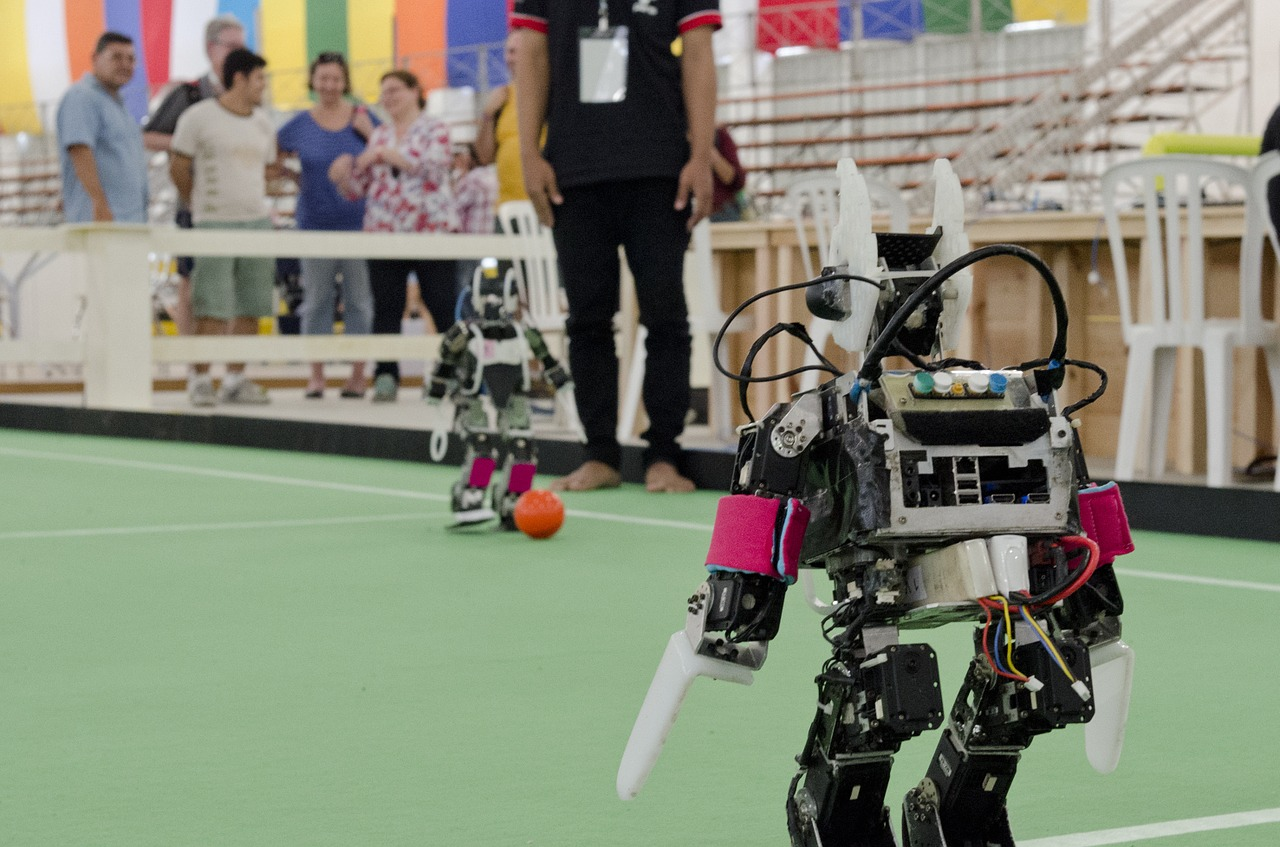
\includegraphics[scale=0.25]{Images/3.jpg}
\caption{Entorno físico del RoboCup}
\end{center}
\end{figure}
En el caso del entorno físico, son los propios “robots” los que tendrán todos los sensores necesarios para la comprensión del entorno, y cada uno de los participantes tendrá la libertad de programarlos de la forma que crea conveniente.

Estos robots tendrán que cumplir con unos parámetros y características específicas para competir de forma justa (o cumplir con un presupuesto máximo en el caso de la RoboCup Rescue).

En ambos casos, tanto en el virtual como en el físico, el comportamiento de los agentes es reactivo. Su función principal consiste en mantenerse a la espera o “patrullando”, según la configuración escogida, en una zona del campo con un gran rango de visión (es decir, sin muchos obstáculos por medio, entendiendo a otros agentes como dichos posibles obstáculos). Estas zonas pueden variar según la situación global, pero el equipo debe seguir manteniendo cierta coherencia para mantener el campo cubierto, aunque los agentes dejen de poder comunicarse entre sí. En el apartado de comunicación se comenta una posible estrategia con esta finalidad.
\section{Problemas técnicos}
En el entorno lógico se darán los problemas ya comentados en el apartado de problemática de un agente físico. En el entorno físico [2], a estos problemas ya comentados se les suman otros problemas que van desde el desarrollo de componentes físicos y baterías que soportan largas partidas, al desarrollo de algoritmos que sean capaces de analizar el entorno y detectar cada elemento a partir de los datos proporcionados por los sensores que incorporan. En el RoboCup tendremos unas regulaciones establecidas para el entorno que siempre serán idénticas, para simplificar el máximo posible el desarrollo de estos algoritmos.

Algunos autores [1] comentan las siguientes líneas de investigación a medio plazo con el fin de solucionar numerosos problemas técnicos que presenta un reto como el RoboCup:
\begin{list}{•}{}
\item Arquitecturas de agentes
\item Reconocimiento, planificación y razonamiento en tiempo real
\item Razonamiento en un entorno dinámico
\item Sistemas multiagentes (en general)
\item Sistemas de percepción
\item Aprendizaje para el desarrollo de tareas complejas
\end{list}

Comparación entre las características del Ajedrez y el RoboCup al ser jugados por agentes inteligentes:
\begin{table}[H]
\begin{center}
\begin{tabular}{| c | c | c| }
\hline
\textbf{Características}  & \textbf{Ajedrez} &\textbf{RoboCup} \\\hline
 \textbf{Entorno} & Estatico & Dinámico \\
  \textbf{Cambio de estado} & Turno & Tiempo real \\
  \textbf{Acceso a la información} & Completa & Incompleta \\
 \textbf{Control} & Centralizado & Distribuido \\
 \hline
\end{tabular}
\caption{Comparación entre el ajedrez y la RoboCup}
\end{center}

\end{table}

Podemos observar en la tabla anterior la complejidad añadida a la creación del agente en la RoboCup, debido a la gran cantidad de problemas añadidos que tienen respecto a un juego como el Ajedrez, para el cual ya existen agentes capaces de competir contra cualquier humano desde 1996 (Deep Blue).


Como hemos comentado anteriormente, uno de los principales problemas de los agentes físicos en un entorno real es la gran cantidad de información que estos deben procesar y es por ello que será necesario arquitecturas ágiles para dichos entornos. Además, recalcar la importancia de estas arquitecturas ya que estos agentes necesitan razonar en un entorno dinámico en tiempo real y, por tanto, el cómputo que realicen estos robots deberá de estar acotado en el tiempo.

\section{Comunicación e interacción}
El RoboCup es un ambiente muy atractivo para los agentes en tiempo real. En el juego, tenemos dos equipos compitiendo. Cada equipo tiene un objetivo en común, que en este caso es el de ganar el juego. El equipo contrario puede ser visto como un impedimento dinámico de dicho objetivo. 

En este caso, la comunicación e interacción entre agentes consiste en el intercambio de mensajes que se da entre los distintos agentes de un mismo equipo para, por ejemplo, establecer una estrategia empezando por compartir entre ellos sus respectivas posiciones y así no tener una concentración de jugadores en una parte del campo mayor a la necesaria.

Una estrategia que se suele seguir es definir un líder para cada uno de los agentes, al cual se acercarán en caso de que esté lejos (siempre se debe mantener en el campo de visión) y en caso de que esté cerca, los agentes volverán a su zona delimitada inicialmente. Así se evita que haya alguna parte del campo desprotegida, o con una cantidad de agentes demasiado elevada.
\begin{figure}[H]
\begin{center}
\includegraphics[scale=0.5]{Images/campo-tecnico.png}
\end{center}
\caption{Estrategia de posicionamiento de los jugadores mediante líderes.}
\end{figure}

Como podemos observar en la imagen de arriba, el jugador de más a la derecha está yendo a por la pelota. Esto hace que los jugadores más cercanos a él también se acerquen a esta zona, y así sucesivamente. Esto nos permitirá que todos los jugadores del campo estén siempre lo más cerca posible de la pelota sin abandonar su posición y sin dejar ninguna parte del campo sin cubrir. Esta estrategia también evitará la concentración de jugadores en cualquier posición.

Los sensores de cada robot (agente) permiten obtener una visión parcial del entorno. Gracias a la comunicación entre ellos se puede completar esta visión parcial y obtener un entorno mucho más completo y exacto.

Uno de los principales problemas (ya comentados en el apartado de problemas técnicos) es el cómo coordinar los agentes que pertenecen a este sistema para obtener un comportamiento global eficiente. Aunque en algunos casos la coordinación se realiza gracias a un conocimiento total del entorno en el que se desenvuelven, en este caso al tratarse de un entorno demasiado complejo (como ya hemos comentado anteriormente) se vuelve necesario el desarrollo de un diseño multi-agente que permita obtener un comportamiento global coordinado basado en los comportamientos reactivos de los agentes que son controlados o dirigidos por la información local que poseen.
Este comportamiento global aparece por primera vez en el dominio de la RoboCup, como una de las mayores aportaciones ofrecidas por esta iniciativa [14].

Otra práctica habitual a la hora de comunicar a los agentes entre sí es la definición de un líder global de equipo, que en el caso del Soccer se trata del jugador que posee el balón en un momento preciso o que tiene más posibilidades de poseerlo.



\section{Aplicaciones}
\subsection{Robocup Rescue}
\begin{figure}[H]
\begin{center}
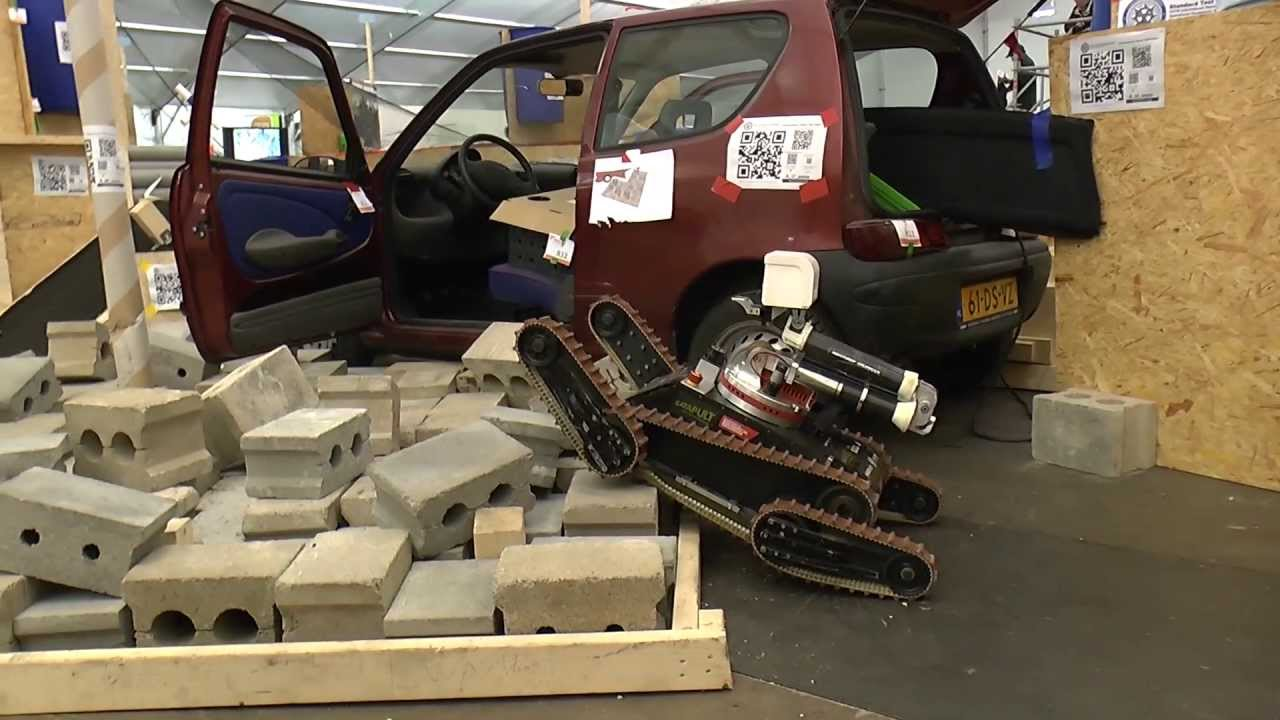
\includegraphics[scale=0.25]{Images/4.jpg}
\caption{Rescate en entorno complejo}
\end{center}
\end{figure}
La idea principal de la RoboCup Rescue reside en el desarrollo de robots para ser utilizados en tareas de rescate ante catástrofes naturales o humanas. Estos robots podrían ser utilizados, por ejemplo, en terremotos para rescatar a personas o recoger víveres.

La RoboCup Rescue supone, por tanto, un importante desafío como competición. Esto es debido a algunas características que se dan en esta modalidad, como la necesidad de trabajo en equipo, el trabajo con información incierta o la necesidad de tiempo real. Además existen otros retos como la gran cantidad de agentes involucrados o la logística, entre otros.


En esta competición distintos robots colaboran para conseguir superar distintas pruebas como \textbf{Sigue líneas}, movimiento de objetos, rescate, etc.
\begin{figure}[H]
\begin{center}
\includegraphics[scale=0.25]{Images/siguelineas.jpg}
\caption{Ejemplo prueba robot sigue líneas}
\end{center}
\end{figure}
Como hemos comentado anteriormente, el objetivo final de esta competición es desarrollar robots que colaboran entre ellos para conseguir operar en zonas donde haya ocurrido una catástrofe. Algunos autores [5] comentan una posible solución a este problema. En primera instancia, ante una catástrofe existe una recogida de datos (mediante drones, satélites etc.) y un posterior procesamiento para realizar una simulación de la catástrofe. Tras esto se pasaría la información al centro de mando donde los operarios pondrían en marcha los robots de rescate (dándoles las instrucciones pertinentes). Estos robots podrían tener funciones como colaborar con los humanos en la retirada de escombros, transporte de heridos, búsqueda de supervivientes, etc.
\begin{figure}[H]
\begin{center}
\includegraphics[scale=0.4]{Images/rescueplan}
\caption{Posible plan para rescate utilizando robots}
\end{center}
\end{figure}
Por tanto, la gran cantidad de robots necesarios en las labores de rescate y su gran diversidad hace que la competición se vuelva un sistema complejo y heterogéneo donde la necesidad de comunicación y colaboración toma un papel importante.

\subsection{Robocup Soccer}
\begin{figure}[H]
\begin{center}
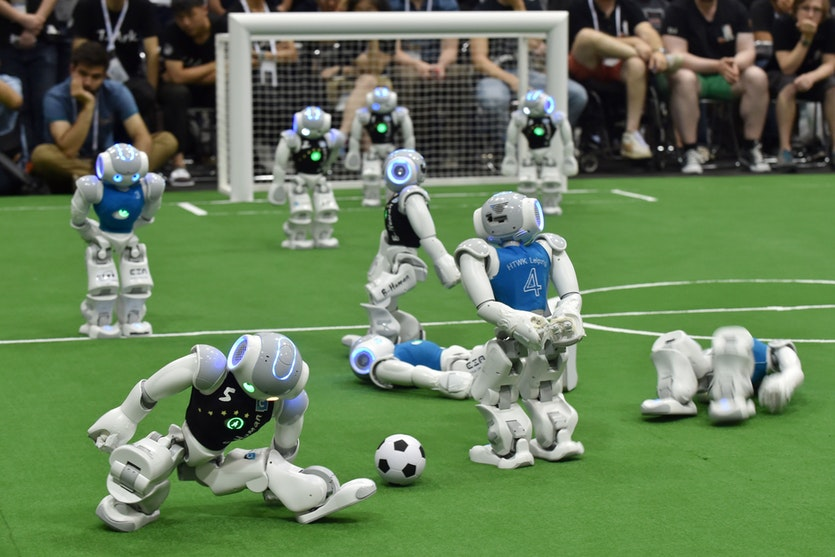
\includegraphics[scale=0.4]{Images/1.jpg}
\caption{Robots jugando al Soccer}
\end{center}
\end{figure}
La RoboCup Soccer consiste en una partida de fútbol entre agentes de 11 contra 11. En ella los robots compiten con el fin de ganar la partida. Estos robots deberán colaborar con otros robots y definir estrategias para vencer a sus contrincantes.

Esta sección fue la primera en aparecer de la RoboCup [3] en el año 1993, cuando fue anunciada la iniciativa y se redactaron las regulaciones. También se anunció este mismo año la versión 0 del primer campo virtual de fútbol donde testear los agentes. Este simulador cuya versión 1.0 fue lanzada en el año 1995 es de código abierto (escrito en C++).


En el año 1997 se realizó el primer evento oficial del RoboCup, que fue exclusivamente para el Soccer y participaron 40 equipos tanto para la parte simulada como para la parte utilizando autómatas. Además al evento asistieron sobre 5.000 espectadores.

A diferencia del RoboCup Rescue, la RoboCup Soccer nace con una perspectiva más lúdica. Además de esto, en comparación, la RoboCup Soccer tiene un entorno más controlado donde el tamaño del campo, color de la pelota, el tamaño de los robots y demás elementos están debidamente definidos y acotados [2]. Un ejemplo de las medidas del campo para una de las ligas se pueden observar en la imagen inferior:

\begin{figure}[H]
\begin{center}
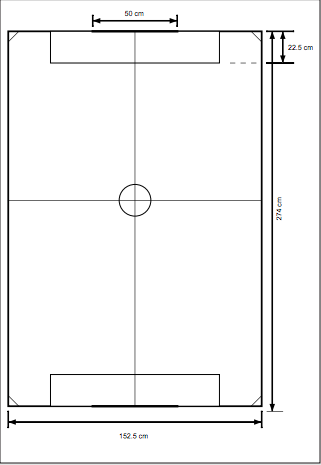
\includegraphics[scale=0.6]{Images/tamano_campo}
\caption{Tamaño reglamentario liga small}
\end{center}
\end{figure}

Las dimensiones del campo así como sus características están condicionadas a las características de los robots. En la RoboCup Soccer se disponen de muchas categorías, las cuales varían en tamaño y proporciones.

En la liga Small, un sistema de visión global sigue en todo momento las posiciones de los robots y la pelota. Este sistema está formado por un conjunto de cámaras situadas a unos 4 metros por encima del campo [9]. Las posiciones son transmitidas a los ordenadores de cada equipo, donde se elaborará la estrategia y será comunicada a los robots habitualmente por radio.
\begin{figure}[H]
\begin{center}
\includegraphics[scale=0.6]{Images/sistema_vision.png}
\caption{Sistema de visión global liga SMALL}
\end{center}
\end{figure}
Un ejemplo práctico de lo comentado anteriormente se puede observar en el grupo de estudiantes y investigadores de la Universidad Carnegie Mellon de Estados unidos, más conocidos como CMDragons. Este equipo ha ganado la liga small durante 5 años (el último 2015) y se ha clasificado quedando en segundo puesto durante otros 4 años.
\begin{figure}[H]
\begin{center}
\includegraphics[scale=0.3]{Images/CMDragons.jpg}
\caption{CMDragons Liga SMALL}
\end{center}
\end{figure}

Como podemos observar en la imagen superior, cada robot tiene en su parte superior un patrón con un código de colores único [10]. Gracias a este patrón y a las cámaras superiores se puede determinar la posición y orientación de cada robot. La posición del robot y de la pelota se transmite a los ordenadores del equipo en los cuales se elabora la estrategia y por último se comunica por radio las nuevas posiciones.

La arquitectura planteada por CMDragons [12] consiste en un módulo de visión que transmite la información a un servidor, el cual distribuye la información a dos clientes mediante sockets UDP: El primer cliente se trata de una interfaz de usuario que permite observar y depurar las jugadas de los robots. El segundo cliente es un programa de Soccer el cual es capaz de realizar una modelización del mundo, así como construir estrategias y tácticas. Estas tácticas serán transmitidas de nuevo al servidor, el cual se encargará de enviarlo por radio al robot.
\begin{figure}[H]
\begin{center}
\includegraphics[scale=0.4]{Images/arq_cmdragons.png}
\caption{Arquitectura planteada por CMDragons}
\end{center}
\end{figure}
En cuanto a la generación de estrategias, algunas situaciones diferenciadas por el equipo [13] son que, por una parte, la estrategia para escoger la mejor localización para realizar un determinado pase consiste en comprobar si se maximiza la probabilidad de marcar el gol si se realiza ese pase.

Por otra parte, definen una estrategia de paso adelantado que consiste en pasar el balón a una determinada posición donde se predice que estará el robot para recibirlo. Con esta estrategia, el equipo trata de minimizar el intervalo de tiempo que tiene el adversario para predecir y bloquear el ataque.

Además, el equipo utiliza análisis probabilístico con el fin de predecir las tácticas utilizadas por el oponente y de esta forma poder anticiparse. Por ejemplo, elaborando una estrategia de defensa con la cual contraatacar.

\begin{figure}[H]
\begin{center}
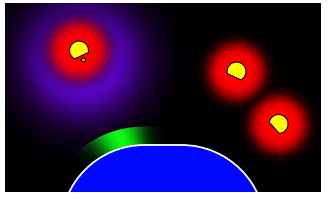
\includegraphics[scale=0.8]{Images/atack_plan.png}
\caption{Plan de ataque CMDragons}
\end{center}
\end{figure}

Por último, disponen de un plan de ataque que consiste en un pase a una determinada posición y un posterior disparo a portería. Para ello se discretizan las posiciones del receptor en una matriz de 6x4 [13] y se evalúa la probabilidad de marcar gol estando en una celda determinada. De esta forma, la celda con mayor probabilidad será donde se realice el pase para ejecutar el plan de ataque.

Por ejemplo, como podemos apreciar en la imagen de la parte superior, el sistema trataría de discretizar la visión del entorno y escoger la mejor posición para maximizar la probabilidad de gol al atacar. Para ello deberá tener en cuenta la mejor posición para el pase y posterior ataque con el fin de evitar la defensa (en color verde) y al portero del equipo oponente.



\subsection{RoboCup  Industrial}
\begin{figure}[H]
\begin{center}
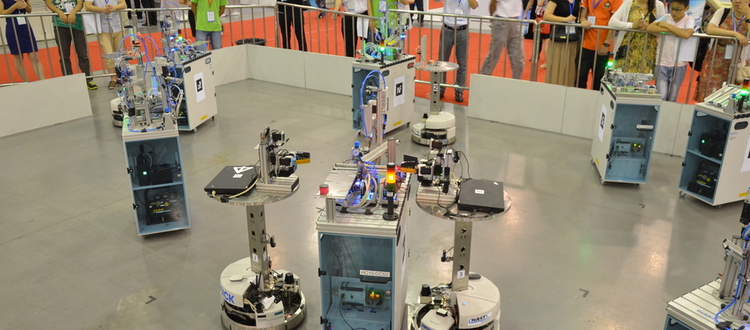
\includegraphics[scale=1.8]{Images/5.png}
\caption{Torneo de la RoboCup Industrial}
\end{center}
\end{figure}
La RoboCup en el ámbito industrial [7] (o RoboCup Logistics League) es una liga impulsada por la utilización de los agentes en la industria. Está enfocada en aquellas fábricas que realizan un proceso poco complejo pero que requiere de personal humano.

La idea es la de permitir la automatización en las fábricas de una forma más económica y que sea posible en ámbitos donde a día de hoy no compensa el beneficio al dinero aportado (por ejemplo producciones para volúmenes reducidos o productos de altas variaciones en las cuales solo robots con una cierta inteligencia son capaces de actuar).
\begin{figure}[H]
\begin{center}
\includegraphics[scale=0.2]{Images/robocup-industrial.jpg}
\caption{Selección de piezas en  RoboCup Industrial}
\end{center}
\end{figure}

Uno de los principales problemas de esta competición es la percepción, en concreto las tareas de segmentación de objetos que se sitúan en una mesa para, por ejemplo, diferenciar entre tornillos y barras. Esto se puede apreciar en la imagen de la parte superior donde el robot necesita distinguir entre las distintas piezas para, por ejemplo, montar una determinada tubería.

Sobre este mismo proyecto ha surgido otro subapartado llamado Work, en el cual se buscan más robots de servicio y apoyo al trabajo. El objetivo final de la competición consiste en desarrollar estrategias de logística, planificación a nivel de tarea y producción en cadena. 
\chapter{Conclusiones}
Como conclusión nos gustaría comentar los siguientes puntos; en primer lugar destacar la gran complejidad que supone diseñar agentes que operan en un entorno dinámico como es el mundo real. La gran cantidad de información que se debe procesar debido a los numerosos sensores que poseen estos robots, la necesidad de trabajar con información incompleta o la complejidad de los algoritmos de logística aumentan notablemente la dificultad de estos agentes.

Otro punto importante que queremos destacar es la necesidad de perfeccionar al máximo el comportamiento global del equipo a partir del perfeccionamiento del comportamiento individual de cada agente en el ámbito de la cooperación entre agentes. Para ello es necesario experimentar con otros equipos en un entorno competitivo, y aquí es donde reside la mayor importancia de este campeonato.

También nos gustaría comentar que pese a la RoboCup tratarse de una organización sin ánimo de lucro, los avances aportados al ámbito de los agentes inteligentes por este proyecto internacional han ayudado al gran progreso de este campo, que todavía está en sus inicios.

En nuestra opinión la RoboCup Soccer es una muy buena iniciativa, pero actualmente resulta poco atractiva para la mayoría de personas. Creemos que un importante avance puede llegar con la competencia añadida y en pleno auge de la RoboCup Home [6], en la cual se busca la integración de los robots autónomos en la vida diaria de las personas. En este caso creemos que puede ser muy interesante para muchas personas ya que la simplificación de las tareas domésticas o rutinarias es algo que todo el mundo busca (como ejemplo tenemos los robots aspiradores, los robots de cocina e incluso los electrodomésticos inteligentes).



\begin{thebibliography}{a}
\bibitem{robocup1} \textsc{The RoboCup Synthetic Agent Challenge 97 },
\textit{http://www.ijcai.org/Proceedings/97-1/Papers/004.pdf}
\bibitem{robocup2} \textsc{RoboCup A Challenge Problem for AI},
\textit{http://www.aaai.org/ojs/index.php/aimagazine/article/download/1276/1177/}
\bibitem{robocup3} \textsc{Robocup},
\textit{http://www.robocup.org/}
\bibitem{phisical} \textsc{Physical Agents},
\textit{https://bisite.usal.es/archivos/agfisicos.pdf}
\bibitem{robocup4} \textsc{RoboCup Rescue},
\textit{\\https://www.aaai.org/ojs/index.php/aimagazine/article/viewFile/1542/1441}
\bibitem{robocup5} \textsc{RoboCup Home},
\textit{http://www.ai.rug.nl/robocupathome/}
\bibitem{robocup6} \textsc{Logistics League},
\textit{$http://wiki.robocup.org/Logistics_League$}
\bibitem{robocup7} \textsc{Work Leaguee},
\textit{$http://wiki.robocup.org/@Work_League$}
\bibitem{robocup7} \textsc{Small Size League},
\textit{$http://wiki.robocup.org/Small_Size_League$}
\bibitem{robocup7} \textsc{CMDragons},
\textit{http://www.cs.cmu.edu/robosoccer}
\bibitem{robocup7} \textsc{CMDragons},
\textit{http://www.cs.cmu.edu/robosoccer}
\bibitem{robocup7} \textsc{CMDragons YouTube},
\textit{https://www.youtube.com/channel/UCK3nZZO46ZAPIh-BoyoQF8Q/videos}
\bibitem{robocup7} \textsc{CMDragons 2010 Extended Team Description},
\textit{https://goo.gl/TqhGvA}
\bibitem{robocup7} \textsc{CMDragons 2014 Team Description},
\textit{https://goo.gl/d4tJk9}
\bibitem{robocup7} \textsc{Coordinación global basada en controladores locales reactivos en la
RoboCup},
\textit{https://goo.gl/2tNuEE}



\newpage
\textbf{\\\\\\Otras consultas:}
\bibitem{robocup6} \textsc{Comprensión sobre los agentes en un entorno simulado},
\textit{https://goo.gl/cNTAao}
\bibitem{robocup7} \textsc{Comprensión sobre los agentes en un entorno simulado},
\textit{https://goo.gl/Fg38fH}
\bibitem{robocup8} \textsc{Comprensión sobre la modalidad RoboCup Home},
\textit{https://www.youtube.com/watch?v=YpjeNa8BAYg}
\bibitem{robocup8} \textsc{\textbf{ Vídeo de presentación}},
\textit{https://www.youtube.com/watch?v=IDPzxaqCnk4}
\end{thebibliography}

\end{document}
